\documentclass[11pt]{article}
\usepackage{amsmath, amssymb, amscd, amsthm, amsfonts}
\usepackage{graphicx}
\usepackage{hyperref}
\usepackage[numbers]{natbib}
\usepackage[utf8]{inputenc}
\usepackage[T1]{fontenc}
\usepackage{subcaption}
\usepackage{multirow}  % Für die Zellen, die mehrere Zeilen überspannen


\oddsidemargin 0pt
\evensidemargin 0pt
\marginparwidth 40pt
\marginparsep 10pt
\topmargin -20pt
\headsep 10pt
\textheight 8.7in
\textwidth 6.65in
\linespread{1.2}

\title{\Large \textbf{Parametersensitivität eines erregbaren Genregulationsnetzwerks:}\\
\Large Eine quantitative Analyse der Kompetenzregulation in \textit{B. subtilis}}

\author{Derya Kilicarslan}
\date{11.05.2025}

\newtheorem{theorem}{Theorem}
\newtheorem{lemma}[theorem]{Lemma}
\newtheorem{conjecture}[theorem]{Conjecture}

\newcommand{\rr}{\mathbb{R}}

\newcommand{\al}{\alpha}
\DeclareMathOperator{\conv}{conv}
\DeclareMathOperator{\aff}{aff}

\begin{document}
\maketitle

\section{Einleitung}\label{section-introduction}

Die Studie von Süel et al. (2006) untersucht die dynamischen Mechanismen der transienten Kompetenz in \textit{Bacillus subtilis} unter Nährstoffmangel– ein temporärer Zustand zur DNA-Aufnahme, der in einer kleinen Subpopulation probabilistisch auftritt.

Die molekulare Grundlage des regulatorische Modul (MeKS) besteht aus drei Hauptkomponenten: dem Transkriptionsfaktor ComK, dem Protein ComS und dem MecA-Komplex. ComK fungiert als Master-Regulator der Kompetenz und unterliegt einer positiven Autoregulation. Seine Aktivität wird durch einen negativen Feedback-Loop reguliert, in dem ComK indirekt die Expression des ComS-Proteins hemmt, welches wiederum den Abbau von ComK verhindert.

Dieses Regulationsnetzwerks kann durch ein mathematisches Modell dargestellt werden. Die Charakterisierung dieses Modells durch Phasenraumanalyse zeigt ein erregbares dynamisches Verhalten mit drei charakteristischen Fixpunkten: einem stabilen Fixpunkt (vegetativer Zustand), einem Sattelpunkt (Schwellenwert) und einem instabilen Spiralpunkt (Kompetenzbereich). Diese Konfiguration entsteht durch die Kombination aus schneller positiver und langsamerer negativer Rückkopplung.

In diesem System können stochastische Fluktuationen ("Rauschen") ausreichen, um temporäre Exkursionen vom vegetativen Zustand in den Kompetenzbereich zu initiieren, ohne dass Bistabilität erforderlich ist. Die Validierung dieses Modells erfolgte durch quantitative Fluoreszenz-Zeitraffer-Mikroskopie, die das transiente Differenzierungsverhalten auf Einzelzellebene bestätigte.

Auf diesem Modell aufbauend untersucht die vorliegende Arbeit, wie Änderungen verschiedener Parameter des Kompetenzschaltkreises die Dynamik des Systems beeinflussen – insbesondere die Robustheit der Parameterwerte für die Erhaltung der Systemerregbarkeit sowie die Dauer der Kompetenzperioden (Tc).

\section{Methoden}\label{section-methods}
\subsection{Implementierung und Analyse des Kompetenz-Modells}

Zur Untersuchung der Kompetenzdynamik wurde das von Süel et al. (2006) \cite{suel2006} beschriebene mathematische Modell verwendet. Das Modell besteht aus zwei gekoppelten gewöhnlichen Differentialgleichung, die die zeitliche Entwicklung der dimensionslosen Konzentration von ComK (\textit{K}) und ComS (\textit{S}) beschreiben: 

\begin{equation}
\frac{dK}{dt} = \alpha_k + \frac{\beta_k K^n}{k_0^n + K^n} - \frac{K}{1 + K + S}
\end{equation}

\begin{equation}
\frac{dS}{dt} = \frac{\beta_s}{1 + (K/k_1)^p} - \frac{S}{1 + K + S}
\end{equation}
\\

Die Bedeutung und Standardwerte der Parameter sind in Tabelle~\ref{tab:standardparameter} zusammengefasst. 

\begin{table}[htbp]
\centering
\caption{Standardparameterwerte für das Kompetenz-Modell}
\label{tab:standardparameter}
\begin{tabular}{lll}
\hline
Parameter & Beschreibung & Wert \\
\hline
$\alpha_k$ & Basale ComK-Expressionsrate & 0,004 \\
$\beta_k$ & Max. ComK-Feedback-Rate & 0,07 \\
$\beta_s$ & ComS-Expressionsrate & 0,82 \\
$k_0$ & ComK-Aktivierungsschwelle & 0,2 \\
$k_1$ & ComS-Repressionsschwelle & 0,222 \\
$n$ & Hill-Koeffizient (ComK) & 2 \\
$p$ & Hill-Koeffizient (ComS) & 5 \\
\hline
\end{tabular}
\end{table}

Dabei wurden die Modelle in Python 3.9.2 implementiert, unter Verwendung der wissenschaftlichen Bibliotheken NumPy (v1.26.4) für numerische Berechnungen, SciPy (v1.13.1) für die Differentialgleichungslösungen und Matplotlib (v3.8.4) für die Visualisierungen. Die Phasenraumanalyse und Fixpunktcharakterisierung wurden mithilfe der SciPy-Bibliothek durchgeführt.

\subsection{Globale Parameteranalyse}
In Anlehnung an Schultz et al. (2007) \cite{schultz2007} wurde eine systematische Untersuchung des Parameterraums durchgeführt. Es wurden 500.000 zufällige Parameterkombinationen generiert, wobei die Parameter aus folgenden Bereichen gezogen wurden:

\begin{itemize}
    \item \( n, p \in \{2, 3, 4, 5\} \)
    \item \( \alpha_k \in [0{,}001; 0{,}05] \)
    \item \( \beta_k \in [0{,}05; 0{,}5] \)
    \item \( \beta_s \in [0{,}6; 1{,}3] \)
    \item \( k_0, k_1 \in [0{,}2; 0{,}8] \)
\end{itemize}

Ein Parametersatz wurde als ``erregbar'' klassifiziert, wenn folgende Kriterien erfüllt waren: (i) genau ein stabiler Fixpunkt bei niedrigem ComK (K < 0,3) existierte, (ii) mindestens ein Sattelpunkt vorhanden war, und (iii) mindestens drei Fixpunkte insgesamt identifiziert wurden. Diese Konfiguration erlaubt Trajektorien, die nach Überschreiten einer Schwelle eine große Exkursion durch den Phasenraum durchlaufen, bevor sie zum stabilen Fixpunkt zurückkehren.

\subsection{Detaillierte Analyse der $\beta_k$-$\beta_s$-Parameterebene}
Um den Einfluss der Schlüsselparameter $\beta_k$ (ComK-Feedback-Stärke) und $\beta_s$ (ComS-Expressionsrate) auf die Erregbarkeit zu untersuchen, wurde ein hochaufgelöster Scan der $\beta_k$-$\beta_s$-Parameterebene durchgeführt. Dabei wurden alle anderen Parameter auf ihre Standardwerte fixiert (Tabelle 1). Die $\beta_k$-$\beta_s$-Ebene wurde mit einer Auflösung von $50 \times 50$ Punkten im Bereich $\beta_k \in [0,05; 0,1]$ und $\beta_s \in [0,6; 1,0]$ abgetastet.

Zusätzlich wurde ein erweiterter Scan mit $\beta_k \in [0,01; 0,3]$ und $\beta_s \in [0,1; 2,0]$ durchgeführt, um die Robustheit des erregbaren Verhaltens in einem größeren Parameterbereich zu evaluieren. Für jede Parameterkombination wurde die Stabilität der Fixpunkte bestimmt und die Größe der erregbaren Region quantifiziert.

\subsection{Hill-Koeffizienten-Analyse}
Die Hill-Koeffizienten $n$ und $p$ charakterisieren die Kooperativität der Bindung von ComK an seinen eigenen Promotor bzw. die Repression von ComS durch ComK. Um ihren Einfluss auf die Robustheit der Erregbarkeit zu untersuchen, wurde für jede Kombination von $n, p \in \{2, 3, 4, 5\}$ die Größe der erregbaren Region in der $\beta_k$-$\beta_s$-Parameterebene bestimmt. Dies ermöglichte die Identifikation von Hill-Koeffizienten-Kombinationen, die eine maximale Robustheit des erregbaren Verhaltens gewährleisten.

Die quantitative Analyse der erregbaren Regionen umfasste die Berechnung der relativen Größe der Region im Parameterraum, der Grenzen der erregbaren Region (minimale und maximale Werte von $\beta_k$ und $\beta_s$) sowie des Abstands der Standardparameter von diesen Grenzen. Diese Maße dienten als Indikatoren für die strukturelle Robustheit des Systems aus einer funktionellen Modellansicht.

\subsection{Stochastische Simulationen}
Zur Untersuchung des Einflusses intrinsischer Fluktuationen auf die Kompetenzdynamik wurde das deterministische Modell um einen stochastischen Term erweitert. Dabei wurde speziell die ComS-Dynamik mit einer additiven Rauschkomponente modelliert:

\begin{equation}
\frac{dS}{dt} = \frac{\beta_s}{1 + (K/k_1)^p} - \frac{S}{1 + K + S} + A \cdot \eta(t)
\end{equation}
\\
wobei $\eta(t)$ einen Ornstein-Uhlenbeck-Prozess darstellt, der durch folgende stochastische Differentialgleichung beschrieben wird:

\begin{equation}
d\eta(t) = \theta \cdot (\mu - \eta(t)) \cdot dt + \sigma \cdot dW(t)
\end{equation}

Hier ist $\theta = 1,0$ die Rückkehrrate zum Mittelwert, $\mu = 0$ der Mittelwert des Prozesses, $\sigma = 0,3$ die Rauschamplitude und $dW(t)$ das Inkrement eines Wiener-Prozesses. 

Die numerische Integration erfolgte mit einer modifizierten Euler-Methode. In jedem Zeitschritt wurde zunächst der deterministische Teil der Gleichungen integriert, und dann der stochastische Term für den Rauschprozess separat berechnet und zur ComS-Dynamik addiert:

\begin{align}
K_{i+1} &= K_i + \frac{dK}{dt}(K_i, S_i) \cdot \Delta t \\
\eta_{i+1} &= \eta_i + \theta \cdot (\mu - \eta_i) \cdot \Delta t + \sigma \cdot \sqrt{\Delta t} \cdot \mathcal{N}(0,1) \\
S_{i+1} &= S_i + \frac{dS}{dt}(K_i, S_i) \cdot \Delta t + \eta_{i+1} \cdot \Delta t \cdot A
\end{align}

wobei $\mathcal{N}(0,1)$ eine standardnormalverteilte Zufallsvariable ist. Es wurde eine Schrittweite von $\Delta t = 0,01$ und eine Simulationsdauer von $t_{max} = 500$ (in dimensionslosen Zeiteinheiten) verwendet. Für jede Parameterkombination wurden 50 unabhängige Simulationen durchgeführt, um statistische Robustheit zu gewährleisten. Nach jeder Integration wurden negative Werte auf Null gesetzt, um die biologische Plausibilität zu wahren.

\subsection{Verstärkungsfaktoranalyse}
Um den optimalen Verstärkungsfaktor $A$ zu bestimmen und den Einfluss der Rauschintensität systematisch zu untersuchen, wurde eine Verstärkungsfaktoranalyse durchgeführt. Hierbei wurde der stochastische Term in der ComS-Gleichung mit verschiedenen Faktoren $A \in \{1, 3, 5, 7, 10\}$ multipliziert:

\begin{equation}
\frac{dS}{dt} = \frac{\beta_s}{1 + (K/k_1)^p} - \frac{S}{1 + K + S} + A \cdot \eta(t)
\end{equation}
\\
Die Wahl des Verstärkungsfaktors $A = 10$ für die Hauptanalysen erfolgte basierend auf dem Vergleich der resultierenden Kompetenzdauern mit experimentellen Beobachtungen aus den Arbeiten von Çağatay et al. (2009) \cite{cagatay2009} und Süel et al. (2006) \cite{suel2006}. Bei diesem Verstärkungsfaktor zeigten die Simulationen Kompetenzdauern, die den experimentell ermittelten 10-20 Stunden (in skalierten Zeiteinheiten) am besten entsprachen. Die Verstärkung des Rauschens diente zudem dazu, die Häufigkeit von stochastisch induzierten Übergängen vom vegetativen zum kompetenten Zustand zu erhöhen, was eine umfassendere statistische Analyse der Kompetenzdauer ermöglichte.

Für jeden Verstärkungsfaktor $A$ wurden 100 unabhängige Simulationen mit einer Dauer von jeweils $t_{max} = 500$ durchgeführt, um eine robuste statistische Basis zu schaffen. 

In einem alternativen Ansatz wurde ein initialer Boost der ComS-Konzentration implementiert und getestet:
\begin{equation}
S(t=0) = S_{basal} \cdot B
\end{equation}
wobei $B$ der Boost-Faktor ist. Verschiedene Boost-Faktoren im Bereich von 5-10 wurden evaluiert, und ein Faktor von $B = 10$ wurde für weitere Analysen ausgewählt. Dieser Ansatz basiert auf experimentellen Beobachtungen, dass Fluktuationen in der ComS-Konzentration hauptsächlich für die Auslösung von Kompetenzereignissen verantwortlich sind (\cite{maamar2007, suel2006}). 

Für beide Ansätze wurde die Kompetenzdauer als die Zeitspanne definiert, in der die ComK-
Konzentration einen Schwellenwert von 0,5 überschritt. Die statistische Analyse umfasste die Berech-
nung der mittleren Kompetenzdauer, der Variabilität der Dauer (Variationskoeffizient) sowie der Ko-
rrelation zwischen Häufigkeit und Dauer der Kompetenzereignisse bei verschiedenen Verstärkungsfak-
toren. Diese systematische Analyse ermöglichte es, den optimalen Verstärkungsfaktor zu identifizieren,
der sowohl realistische Kompetenzdynamik erzeugt als auch ausreichend Ereignisse für eine robuste
statistische Auswertung liefert.

\section{Ergebnisse}\label{section-results}

\subsection{Verteilung erregbarer Parameterkonfigurationen}

Die systematische Analyse des Parameterraums identifizierte eine signifikante Anzahl erregbarer Konfigurationen unter den 500.000 untersuchten Parametersätzen (s. Abb.~\ref{fig:param_histograms}). In der Verteilung der Hill-Koeffizienten zeigt sich eine Tendenz, insbesondere für den Koeffizienten $p$, der ein Maximum bei $p=5$ aufweist, was dem Standardwert aus dem Modell entspricht. Des Weiteren lässt sich erkennen, dass außer der basalen Expression von ComK $\alpha_k$ die Histogramme eine breite, gaußähnliche Verteilung aufweisen (vgl. \cite{schultz2007}). Die Verteilung von $\alpha_k$ ist deutlich schmaler und konzentriert sich nahe dem Standardwert von 0,004. Die ComK-Feedback-Stärke $\beta_k$ und die ComS-Expressionsrate $\beta_s$ zeigen breitere Verteilungen, wobei die jeweiligen Standardwerte innerhalb dieser Verteilungen liegen. Ähnlich verhält es sich mit den Aktivierungs- und Repressionsschwellen $k_0$ und $k_1$.


\begin{figure}[h]
    \centering
    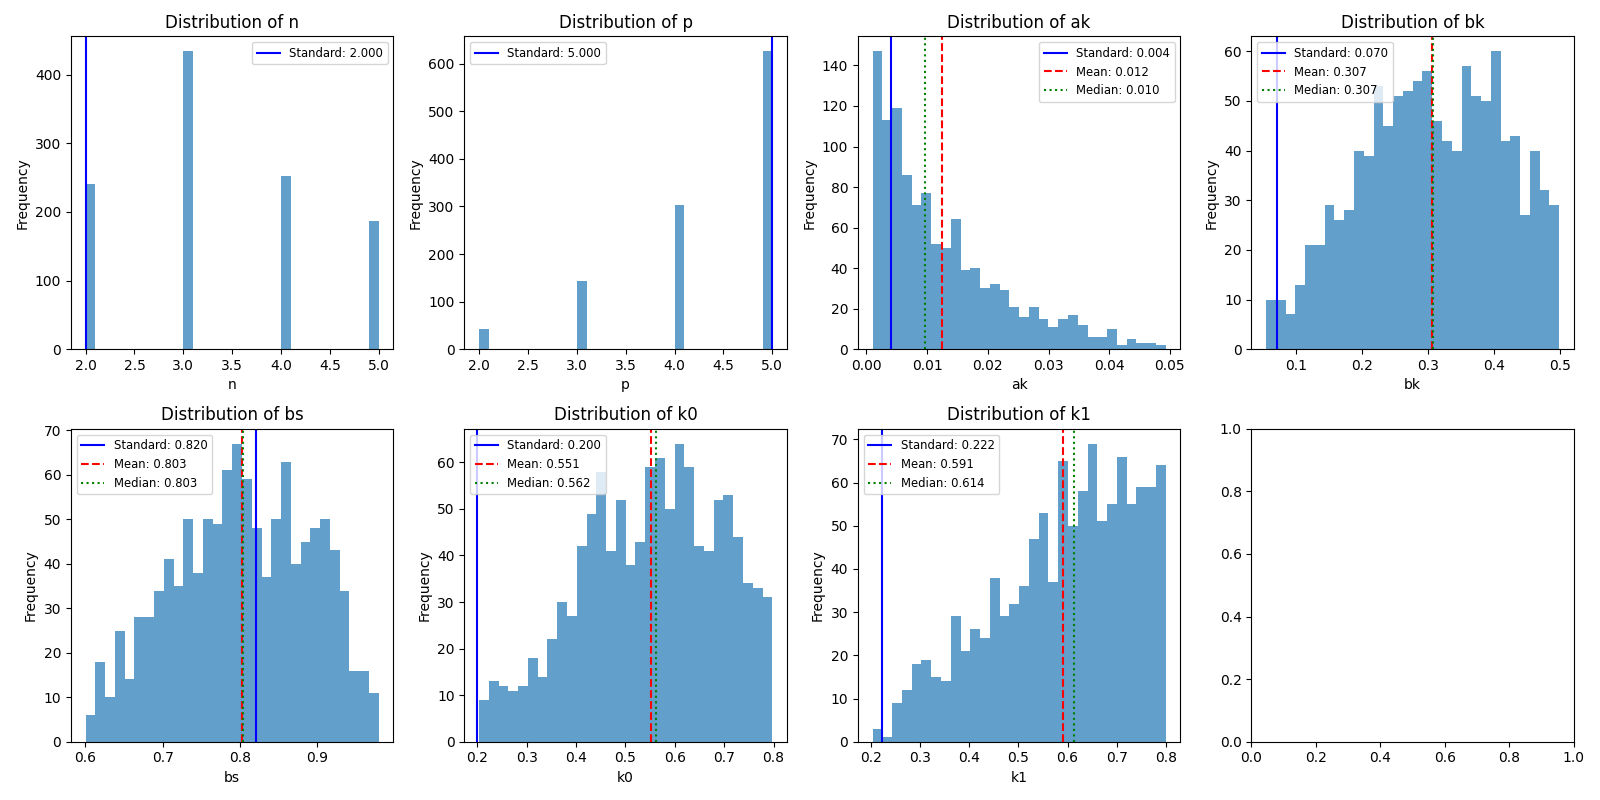
\includegraphics[width=\textwidth]{figures/parameter_histograms.png}
    \caption{Verteilung der Parameterwerte für erregbare Konfigurationen. Gezeigt sind Histogramme für jeden Parameter des Modells ($n$, $p$, $\alpha_k$, $\beta_k$, $\beta_s$, $k_0$, $k_1$). Die vertikalen Linien markieren die Standardwerte (blau), Mittelwerte (rot gestrichelt) und Medianwerte (grün gepunktet) der Verteilungen. Das letzte Diagramm zeigt ein Beispiel für Nullklinen bei einer repräsentativen erregbaren Konfiguration.}
    \label{fig:param_histograms}
\end{figure}

\subsection{Einfluss von Hill-Koeffizienten auf die Erregbarkeit des Kompetenz-Schaltkreises}
Die Parameter $\beta_k$ (ComK-Feedback-Stärke) und $\beta_s$ (ComS-Expressionsrate) beeinflussen kritisch die Dynamik des Kompetenz-Schaltkreises. Die Phasendiagramme in Abb.~\ref{fig:phase-bk-bs} zeigen die erregbaren Regionen im $\beta_k$/$\beta_s$-Parameterraum für verschiedene Hill-Koeffizienten.

\begin{figure}
    \centering
    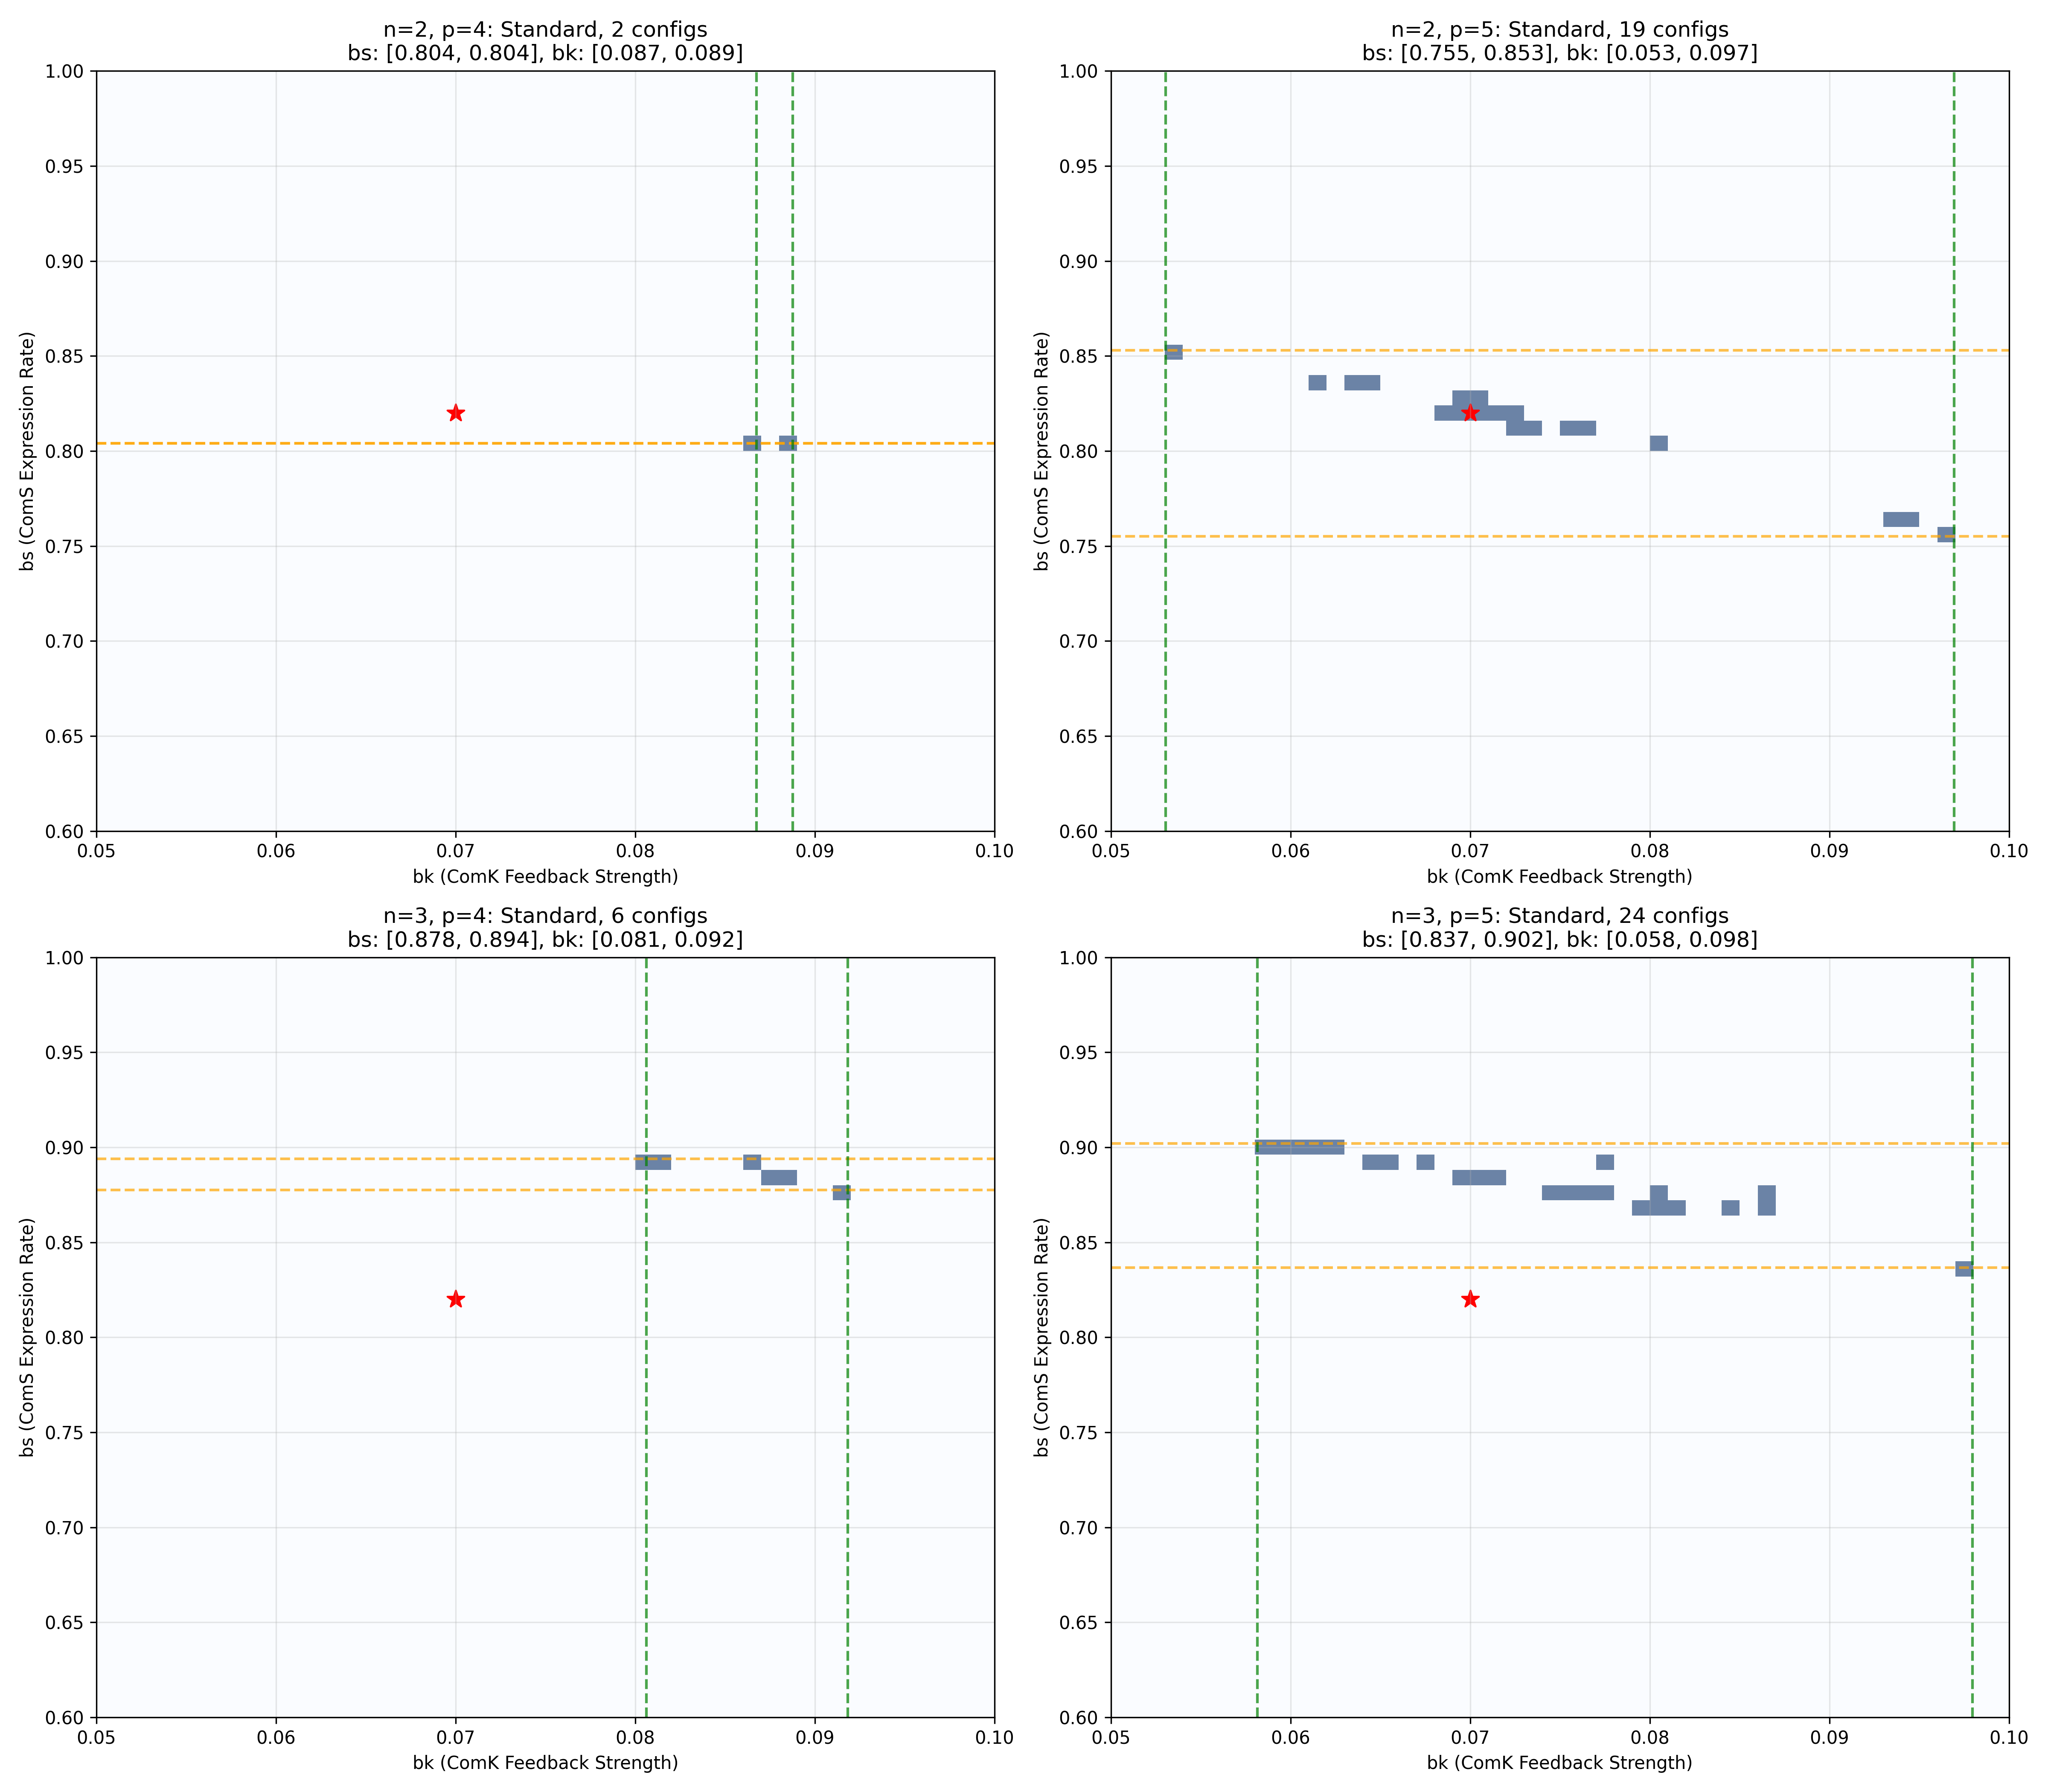
\includegraphics[width=\textwidth]{figures/phase_diagram_with_boundaries.png}
    \caption{Erregbare Regionen im $\beta_k$/$\beta_s$-Parameterraum für verschiedene Hill-Koeffizienten-Kombinationen. Die Plots zeigen die erregbaren Konfigurationen (blaue Quadrate) für (a) $n=2$, $p=4$, (b) $n=2$, $p=5$ (Standard-System), (c) $n=3$, $p=4$ und (d) $n=3$, $p=5$. Der rote Stern kennzeichnet den Standardparametersatz ($\beta_s=0.82$, $\beta_k=0.07$).}
    \label{fig:phase-bk-bs}
\end{figure}

Die Kombinationen mit $p=4$ zeigen deutlich kleinere erregbare Regionen, mit nur 2 Konfigurationen für $n=2, p=4$ und 6 Konfigurationen für $n=3, p=4$.
Für die Standardkombination ($n=2$, $p=5$) liegt die erregbare Region bei $\beta_s \in [0.755, 0.853]$ und $\beta_k \in [0.053, 0.097]$. Der Standardparametersatz ($\beta_s=0.82$, $\beta_k=0.07$) liegt zentral in dieser Region, was optimale Robustheit gewährleistet.

Für $n=3$ verschieben sich die erregbaren Regionen zu höheren $\beta_s$-Werten: $\beta_s \in [0.878, 0.894]$ für $p=4$ und $\beta_s \in [0.837, 0.902]$ für $p=5$.
Obwohl die Kombination $n=3$ und $p=5$ eine höhere Anzahl erregbarer Konfigurationen (24) zeigt, ist der variable Bereich für $\beta_s$ etwas schmaler, während der Bereich für $\beta_k$ ähnlich ist. Darüber hinaus kann in dieser Kombination für die Standartwerte von $\beta_s$ und $\beta_s$ kein erregbares System beobachtet werden.

\subsection{Parameterabhängige Kompetenzdauer und Anstiegszeiten}

\begin{figure}
    \centering
    % Erstes Bild (ohne Boost)
    \begin{subfigure}{\textwidth}
        \centering
        \includegraphics[width=0.9\textwidth]{figures/boxplot_comparison_no_boost.png}
        \caption{Vergleich ohne Boost, Amplifikationsfaktor 10}
        \label{fig:boxplot_no_boost}
    \end{subfigure}
    
    \vspace{0.3cm} % Reduzierter Abstand zwischen den Bildern
    
    % Zweites Bild (mit Boost)
    \begin{subfigure}{\textwidth}
        \centering
        \includegraphics[width=0.9\textwidth]{figures/boxplot_comparison_boost_5amp.png}
        \caption{Vergleich mit Boost 10, Amplifikationsfaktor 5}
        \label{fig:boxplot_with_boost}
    \end{subfigure}
    
    \caption{Vergleich der Kompetenzdauer und Anstiegszeiten für verschiedene Parametersets. \textbf{Links:} Kompetenzdauer. \textbf{Rechts:} Anstiegszeiten. (\subref{fig:boxplot_no_boost}) ohne Boost (Amplifikationsfaktor 10), (\subref{fig:boxplot_with_boost}) mit Boost 10 (Amplifikationsfaktor 5). Die Medianwerte (orange Linien), Interquartilbereiche und Ausreißer zeigen deutliche Unterschiede zwischen den Konfigurationen.}
    \label{fig:boxplot_comparison}
\end{figure}

Die stochastische Analyse der Kompetenzschaltkreisdynamik (Abb.~\ref{fig:boxplot_comparison}) offenbart deutliche Unterschiede in der Kompetenzdynamik in Abhängigkeit von den initialen Simulationsbedingungen. Vergleicht man die Ergebnisse ohne initialen ComS-Boost (Abb.~\ref{fig:boxplot_no_boost}) mit denen mit 10-fachem initialen ComS-Boost (Abb.~\ref{fig:boxplot_with_boost}), zeigen sich markante Veränderungen in den Kompetenzparametern.

Ohne ComS-Boost weisen die exzitablen Konfigurationen 3, 6 und 4 deutlich längere Kompetenzereignisse auf (Median: 74,5-83,2), während Standardparameter und modifizierte Einzelparameter zu kürzeren Kompetenzereignissen führen (Median: 13,6-19,2). Der 10-fache ComS-Boost führt zu einer bemerkenswerten Umstrukturierung der Kompetenzcharakteristiken (Tab.~\ref{tab:boost-comparison}): Die Kompetenzdauer der exzitablen Konfigurationen verringert sich drastisch auf 18,2-18,5, was einer Reduktion um 75-78\% entspricht. Im Gegensatz dazu ist der Effekt auf die Standardparameter und modifizierten Einzelparameter weniger ausgeprägt, mit Reduktionen zwischen 10-35\%.

\begin{table}[h]
    \centering
    \caption{Vergleich der Medianwerte ohne Boost (AF 10) und mit Boost (AF 5).}
    \label{tab:boost-comparison}
    \begin{tabular}{lccccccc}
        \hline
        \multirow{2}{*}{\textbf{Parameterset}} & 
        \multicolumn{3}{c}{\textbf{Ohne Boost (Amp. 10)}} & 
        \multicolumn{3}{c}{\textbf{Mit Boost 10 (Amp. 5)}} \\
        \cline{2-7}
        & \textbf{Duration} & \textbf{Rise} & \textbf{Ratio} & 
        \textbf{Duration} & \textbf{Rise} & \textbf{Ratio} \\
        \hline
        Standard & 16.76 & 11.05 & 0.641 & 10.91 & 5.96 & 0.575 \\
        Excitable Config 3 & 74.50 & 30.93 & 0.473 & 18.15 & 8.82 & 0.547 \\
        Excitable Config 6 & 83.16 & 30.67 & 0.407 & 18.46 & 8.61 & 0.516 \\
        High ComK Basal (2x) & 13.63 & 8.60 & 0.661 & 8.76 & 5.13 & 0.577 \\
        High ComK Feedback (1.5x) & 14.87 & 9.45 & 0.686 & 10.83 & 6.48 & 0.623 \\
        High ComS Expression (1.5x) & 19.19 & 13.04 & 0.672 & 12.50 & 7.47 & 0.596 \\
        Low ComS Expression (0.75x) & 16.66 & 11.63 & 0.673 & 15.04 & 7.79 & 0.597 \\
        \hline
    \end{tabular}
\end{table}

Besonders aufschlussreich ist das Verhältnis zwischen Anstiegszeit und Gesamtdauer. Ohne Boost zeigen die exzitablen Parametersätze mit langen Kompetenzereignissen deutlich niedrigere Rise/Duration-Verhältnisse (0,41-0,47), während Sets mit kurzen Ereignissen höhere Verhältnisse aufweisen (0,64-0,69). Mit initialem ComS-Boost gleicht sich dieses Verhältnis stärker an: exzitable Konfigurationen erreichen Werte von 0,52-0,55, während die übrigen Parametersätze ihr Verhältnis nur leicht reduzieren (0,57-0,62).

Eine detailliertere Analyse der Wahrscheinlichkeitsdichteverteilungen der Kompetenzdauer (Abb.~\ref{fig:kde_comparison}) veranschaulicht zusätzlich die Auswirkungen des initialen ComS-Boosts. Ohne Boost zeigen die Standardparameter und modifizierten Einzelparameter relativ schmale Verteilungen mit Maxima zwischen 10-15 Zeiteinheiten, während die exzitablen Konfigurationen deutlich breitere Verteilungen mit längeren Schwänzen in Richtung höherer Dauern aufweisen.

Mit 10-fachem ComS-Boost verschieben sich sämtliche Verteilungen zu kürzeren Dauern, und auffällig ist die deutlich stärkere Konzentration der Wahrscheinlichkeitsdichte bei niedrigeren Werten, besonders ausgeprägt bei den hochregulierten ComK-Expressionen (High ComK Basal, High ComK Feedback). Bemerkenswert ist auch, dass die exzitablen Konfigurationen 3 und 6, die ohne Boost die längsten Kompetenzereignisse zeigten, unter Boost-Bedingungen deutlich kompaktere Verteilungen mit kürzeren Maximalwerten aufweisen – ein Hinweis auf eine grundlegende Veränderung ihrer Dynamik.

\begin{figure}[htbp]
    \centering
    % Erstes Bild (ohne Boost)
    \begin{subfigure}{0.48\textwidth}
        \centering
        \includegraphics[width=\textwidth]{figures/duration_kde_no_boost_amp10.png}
        \caption{Ohne Boost, Amplifikationsfaktor 10}
        \label{fig:kde_no_boost}
    \end{subfigure}
    \hfill % Fügt einen horizontalen Abstand zwischen den Bildern ein
    % Zweites Bild (mit Boost)
    \begin{subfigure}{0.48\textwidth}
        \centering
        \includegraphics[width=\textwidth]{figures/duration_kde_with_boost_amp5.png}
        \caption{Mit Boost 10, Amplifikationsfaktor 5}
        \label{fig:kde_with_boost}
    \end{subfigure}
    
    \caption{Wahrscheinlichkeitsdichteverteilungen (KDE) der Kompetenzdauer für verschiedene Parametersätze. (\subref{fig:kde_no_boost}) breitere Verteilungen und längere Kompetenzdauern (\subref{fig:kde_with_boost}) schmalere Verteilungen mit stärkerer Konzentration bei kürzeren Kompetenzdauern}
    \label{fig:kde_comparison}
\end{figure}

\section{Diskussion}\label{section-discussion}

\subsection{Allgemeine Parametersensibilität}

Die Ergebnisse der Parameterraumanalyse deuten auf eine Region im Parameterraum hin, die kompakt und groß genug ist, um robust gegenüber Parameterschwankungen zu sein. Die schmale Verteilung von $\alpha_k$ weist auf eine höhere Sensitivität des Systems gegenüber Änderungen in diesem Parameter hin, während die breiteren Verteilungen von $\beta_k$, $\beta_s$, $k_0$ und $k_1$ eine gewisse Robustheit gegenüber Parametervariationen aufzeigen. Diese Robustheit könnte ein wichtiges Merkmal des biologischen Systems sein, das es \textit{B. subtilis} ermöglicht, unter verschiedenen Umweltbedingungen zuverlässig in den Kompetenzzustand zu wechseln, während gleichzeitig die basale ComK-Expression strenger kontrolliert werden muss, um ungewollte Kompetenzinitiierung zu vermeiden.

\subsection{Analyse der ComK-Feedback und ComS-Expression Interaktion unter verschiedenen Hill-Koeffizienten}

Die Untersuchung zum Einfluss der Hill-Koeffizienten bestätigt und erweitert die Erkenntnisse von Süel et al.\ \cite{suel2006} zur Funktionsweise des Kompetenznetzwerks. Höhere Hill-Koeffizienten, insbesondere für die ComS-Repression (\( p = 5 \)), erzeugen robustere erregbare Systeme. Das unterstreicht die kritische Bedeutung der nichtlinearen ComS-Repression für die Systemrobustheit.

Darüber hinaus existiert die Erregbarkeit des Systems in  klar definierter Parametergrenzen. Bei der ComS-Expression (\( \beta_s \)) verhindert eine zu niedrige Rate die ausreichende Hemmung des ComK-Abbaus, wodurch keine Kompetenzinitiierung stattfinden kann; oberhalb eines Schwellenwerts wechselt das System in bistabiles Verhalten. Ähnlich verhält es sich mit der ComK-Rückkopplungsstärke (\( \beta_k \)): Unzureichende Werte generieren nicht die nötige positive Rückkopplung für die Initiierung der Kompetenz.

Dieser begrenzte Parameterraum erklärt möglicherweise, warum nur ein Teil der Zellen (10--15\,\%) \cite{maier2008, cagatay2009, leisner2009, maamar2007} unter Stressbedingungen in den Kompetenzzustand übergeht. 

Weiter interessant zu analysieren wäre die Einführung einer Zeitverzögerung (\( \tau \)) bei der ComS-Repression - im Supplement von Süel et al. wird dokumentiert, dass dies den Instabilitätsbereich des kompetenten Fixpunkts substantiell vergrößert und die Systemerregbarkeit bei reduzierten Hill-Koeffizienten aufrechterhält. Diese Erweiterung des erregbaren Regimes ermöglicht stochastischen Fluktuationen, in einem größeren Parameterbereich erfolgreich Kompetenz auszulösen, was die Robustheit des Systems erhöht.

\subsection{Kompetenzdauer}\label{subsection-kompetenzdauer}
In dieser Arbeit wurde ein modifizierter stochastischer Simulationsansatz gewählt, um eine größere Anzahl von Kompetenzereignissen für die statistische Analyse zu generieren. Dabei wurde eine Kalibrierung auf die in den Arbeiten von Süel et al.\ (2006) und Çağatay et al.\ (2009) gemessenen Kompetenzdauern von ca.\ 15--20~h angestrebt. Diese methodische Anpassung ermöglichte eine bessere statistische Auswertung, verhinderte jedoch eine direkte Einschätzung der tatsächlichen Kompetenzinitiierungswahrscheinlichkeit, die ebenfalls Ziel der ursprünglichen Arbeit war.

Die Analyse zeigt eine starke Abhängigkeit der Kompetenzcharakteristiken von der initialen ComS-Konzentration und dem Verstärkungsfaktor des Rauschens. Diese Parameter beeinflussen maßgeblich die Trajektorien im Phasenraum, was sich deutlich in den unterschiedlichen Kompetenzdauern widerspiegelt. Bei exzitablen Konfigurationen führt der 10-fache initiale ComS-Boost zu einer drastischen Verkürzung der Kompetenzdauer um 75--78\,\%, von Medianwerten von 74{,}5--83{,}2 auf 18{,}2--18{,}5 Zeiteinheiten.

Ein weiterer Vergleich mit dem Arbeit von Leisner et al.\ (2009) \cite{leisner2009} beobachteten in Einzelzellexperimenten eine klar definierte Schaltperiode von \( r = 1{,}4 \pm 0{,}3 \,\text{h} \). In den durchgeführten Simulationen wurden jedoch deutlich abweichende Anstiegszeiten festgestellt, die der Kalibrierung nach Süel et al.\ entsprechen. Dort beträgt die Anstiegszeit etwa \( \approx 5\,\text{h} \).

Ohne ComS-Boost zeigen die exzitablen Konfigurationen sehr niedrige Rise/Duration-Verhältnisse (0{,}41--0{,}47), während die Standardparameter höhere Werte aufweisen (0{,}64--0{,}69). Diese Diskrepanz zum theoretischen Modell, das eine schnelle Autoregulation und langsamere Repression vorhersagt, deutet auf Limitationen des modifizierten Simulationsansatzes hin.

Die Analyse der Wahrscheinlichkeitsdichteverteilungen unterstreicht zusätzlich den tiefgreifenden Einfluss der initialen ComS-Konzentration: Mit ComS-Boost zeigen sich deutlich schmalere, konzentriertere Verteilungen im Vergleich zu den breiteren Verteilungen ohne Boost. Dies verdeutlicht, dass die stochastischen Fluktuationen in der ComS-Konzentration eine entscheidende Rolle bei der Initiierung und Charakteristik der Kompetenzereignisse spielen.

Trotz der methodischen Einschränkungen bezüglich der quantitativen Übereinstimmung mit experimentellen Daten demonstrieren die Simulationsergebnisse die grundlegende Bedeutung der ComS-Dynamik für die Kontrolle der Kompetenzdauer in \textit{Bacillus subtilis} und unterstreichen die starke Parametersensitivität dieses erregbaren Genregulationssystems.

\bibliographystyle{plain}
\bibliography{references} % see references.bib for bibliography management

\end{document}
